\chapter{Literature Review}
\label{chp:chapter2}
\graphicspath{{figures/}{figures/chapter2/}}

\section{Overview}

The resilience and connectivity of transport networks are a long-studied
topic within
transportation engineering in both theoretical and practical contexts.
Within this long history
however, there is variability in how scholars define resiliency. There are
three basic
definitions that researchers have used include:

\begin{itemize}
	\item Resilience through Resistance: Resilient transportation networks
	have few and manageable vulnerabilities. This is typically addressed
	through robust facility-level engineering and risk management
	\citep{bradley2007, peeta2010}.
	\item Resilience through Recovery: Resilient transportation networks are
	able to be repaired and returned to normal service without inordinate
	delay. This is accomplished through effective resource allocation and
	incident management during both disaster or degraded operation
	\citep{zhang2016}.
	\item Resilience through Operability in Crisis: Resilient transport
	networks are able to operate effectively with damaged or unusable links
	\citep{berdica2002, ip2011}.
	It is this definition that is most relevant in the context of this study.
\end{itemize}

These definitions are not entirely mutually exclusive, and many
researchers apply more than one
definition in their work. For example, knowing where systemically critical
or vulnerable links
are will help in allocating maintenance resources. At the same time, the
approach to identifying
critical facilities implied by one of these definitions is not always
compatible with the other
definitions, and making distinctions between them is important
\citep{rogers2012}. A bridge
highly vulnerable to failure may be located on a little-traveled and
systemically unimportant
side street. The motivation of this research is to identify systemically
critical facilities, and literature using the third definition is the primary consideration.

To begin, a basic understanding of what resiliency is -- or is not -- needs
to be developed. Professionals, including those at UDOT, have adopted use of
the Four R’s as a means to predict some form of resilience on a highway
network. The Four R’s include: rapidity, redundancy, robustness, and
resourcefulness. In the Four R's, rapidity is inversely related to the closure
time and is heavily used to measure how quickly a road can recover from a
setback such as a minor accident or temporary closure. Redundancy is measured
by the additional time or distance a user has to travel when a route is broken.
Ideally, a highly redundant system has many alternative routes built into
itself such that a user could easily alter their route with little or no
increased travel time or travel distance. Greater amounts of time or distance
lower the overall redundancy. Robustness is the inverse of risk and represents
the overall strength of the system as a whole. Resourcefulness, the last of the
Four R’s, is the ability to find quick solutions in a network.

We begin this review first by examining a study conducted by AEM on
behalf of UDOT to identify
vulnerable sections on the I-15 corridor. Next, we consider observations
learned from systemic
changes to networks and populations under real-life crisis events. We then
consider previous
attempts in the academic literature to evaluate the resiliency of real and fabricated
transportation networks.

\section{Identifying Critical Links on I-15}

AEM worked with UDOT to develop an I-15 Corridor Risk and Resilience
Pilot \citep{aem2017}. This
project had a seven-step plan to understand the impact of physical threats
to the Utah
transportation network, specifically looking at two sections along I-15.
These steps included:

\begin{itemize}
	\item Asset characterization - A method to divide physical road assets into
	groupings with similar characteristics; e.g roads, bridges, culverts, etc.
	\item Threat characterization - A method to determine threat types each asset
	is exposed to or could be affected by; e.g. rock fall, fire, flood, etc.
	\item Consequence analysis - An analysis determining the consequences of link
	loss, primarily estimating the cost of replacement should a link become
	damaged or broken
	\item Vulnerability assessment - An assessment of the amount of vulnerability
	each link is exposed to when single or multiple threat types are present
	\item Threat assessment - A method to determine the realized threat level
	present at each link examined
	\item Risk/Resilience assessment - A measure of the risk level and an attempt
	at a measure of the importance of each link to the roadway as a whole
	\item Risk/Resilience management - A summary of steps that should be taken to
	mitigate immediate risk, and reduce future risk while increasing the
	resilience level of individual road assets
\end{itemize}

From these different steps and assessments,
AEM was able to provide a number of recommendations to UDOT that had the
potential to improve
resilience along the evaluated corridors (mainly sections of I-15)
based on the criticality rating (a combination measure of the information
listed above) determined for each segment at risk.

It is easy to understand just how many natural or man-made threats exist to
current infrastructure. Natural disasters such as earthquakes, wildfire,
landslides and flash-floods cause billions of dollars of damage each year.
Other threats such as terrorism affect important infrastructure as well.
Thus, for the purpose of this thesis, it is important to understand which
threats exist, and which threats AEM decided to analyze.

AEM identified a number of threats which should be considered in Utah, based
on a number of different types of data which was available for use. AEM was
also able to rule out certain types of threats based on the relevance of these
threats in Utah. Ultimately, AEM considered nine physical threats which
include: earthquake, flood (scour), flood
(overtopping/debris), fire
(wild-land), railway-proximity, oil/gas/water pipeline-proximity, and water
canal/ditch-proximity. Data comprising historical disaster occurrences or
geographic location about these threat types exist and was assembled into
threat layers which were intersected with physical assets (roadway,
bridge, etc.).

Once these threat layers were determined and the location of the threat-
asset pairs along I-15
were found, AEM was able to begin their analysis of how at-risk a link or road
segment might be to the nine identified threat types. This process consisted of
gathering characteristic
data for each asset (length, width, depth, condition, etc.), determining a
replacement cost for
each asset, establishing an estimated service life for each asset,
estimating (if not known) the
design standard for each asset, establishing which magnitudes of each
threat were to be analyzed,
and gathering information on the likelihood of occurrence of each
magnitude of each threat. These
steps are further described in the published report.

The AEM Risk and Resilience report provides a good template going forward for identifying
links at risk,
following the first definition of a resilient transportation network. The
report also attempts to
identify which links are most critical, assessing a “criticality”
score to the network
based on the five data elements and categories given in Table \ref{tab:aemscore}.
Table \ref{tab:aemscore} provides insight into the some of the complications involved in
attempting to identify critical roads. For example, a road may have a low AADT, but
the majority of that AADT, which would show that there is a very low to low impact,
however, if the majority of traffic on that road were truck traffic, then that road almost
immediately has a moderate to high impact. Other nuances such as that in the previous
example exist. What would happen in the case that a minor arterial became inundated, however,
there was a redundant arterial just a few blocks or miles away? One other observation made from the
\ref{tab:aemscore} is that AEM does not take alternate routes into account.
AEM does not include a way for their developed risk analysis methodology
to anticipate what a user would actually do if faced with a real disaster
scenario. AEM does not answer simple questions such as how many valid
alternative routes exist? What is the new travel time or travel distance?
Identifying the systemic resiliency of highway facilities
– as implied by the third definition of resiliency, resilience through
operability in crises – requires considering these alternate routes \citep{aem2017}.

\begin{table}

\caption{AEM Criticality Score}
\label{tab:aemscore}
\makebox[\linewidth]{
\centering
\begin{tabular}[t]{llllll}
\toprule
Criteria & Very Low Impact & Low Impact & Moderate Impact & High Impact & Very High Impact\\
\midrule
AADT & $\leq 1,145$ & 1,146-3,275 & 3,276-8,285 & 8,286-17,455 & $>$17,455\\
Truck AADT & 0 & 1-494 & 495-1,881 & 1,882-4,794 & $>$4,794\\
\makecell{AASHTO\\Classification} & \makecell{Minor \\Collectors} & \makecell{Minor \\Collectors} & \makecell{Minor \\Arterials} & \makecell{Principal \\Arterials} & \makecell{Interstate \\Expressway}\\
\makecell{Tourism\\Traffic (\$M)} & $<19.89$ & 19.90-39.66 & 39.67-101.13 & 101.14-505.32 & $>$505.32\\
\makecell{Maintenance\\Distance (Mi)} & $<70$ & 71-84 & 85-102 & 103-124 & $>124$\\
\bottomrule
\end{tabular}
}
\end{table}

\section{Lessons Learned from Crisis Events}

Two major crisis events in the last fifteen years have given researchers
an important opportunity
to study what happens to transportation networks and user behavior when critical links are
suddenly disabled for an
extended period of time. These events are the I-35W bridge
collapse in
Minneapolis, Minnesota, and the I-85 / Piedmont Road fire and bridge
collapse in Atlanta, Georgia.

\subsection{I-35W Bridge Collapse}

On August 1, 2007, the I-35 bridge over the Mississippi River in downtown
Minneapolis collapsed
during rush hour. The bridge, which was undergoing maintenance, had been
rated as structurally
deficient and fracture critical, meaning that failure of one member would
cause structure
failure \citep{schaper2017}. The collapse occurred during rush hour traffic, and the bridge
was additionally loaded
with approximately 300 tons of maintenance equipment \citep{schaper2017}.
There were 13
fatalities,
approximately 140 injuries, and abrupt disruption to roughly 140,000
average daily trips (ADT)
over the bridge \citep{zhu2010}. The complicated nature of the demolition
and repair meant
this systemically critical link would be missing for approximately 14
months. The approximate
location of the bridge, one of two major routes over the Mississippi
River, can be seen in Figure \ref{fig:i35}.

\begin{figure}

{\centering 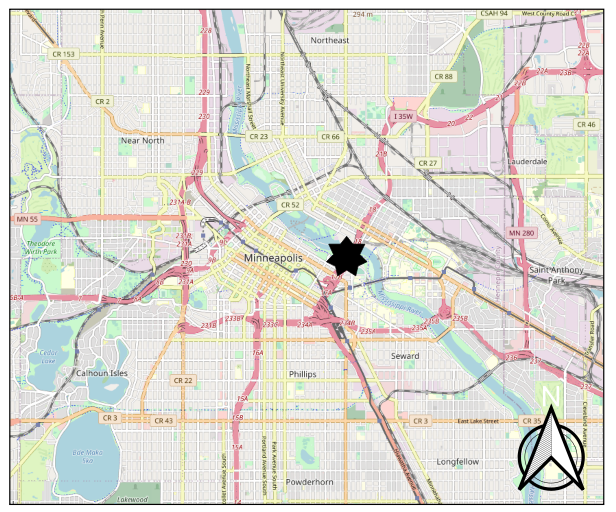
\includegraphics[width=0.75\linewidth]{figures/chapter2/I-35W.png}

}

\caption{Approximate location of the I-35W bridge collapse.}\label{fig:i35}
\end{figure}

\citet{zhu2010} conducts a travel survey to provide a more in-depth
analysis of important data
and traffic changes surrounding the I-35W bridge collapse in 2007. The
article uses a methodology
that attempts to identify mode-choice and other behavioral changes of
survey respondents. The
authors analyze data looking for variations in ADT, as well as origin-destination (OD) matrices.
Importantly, they analyze loop detector data, bus ridership statistics, and survey response data in their work. The
authors conduct a regression analysis of the collected data,
which indicates that drivers are reluctant to make mode choice changes,
rarely doing so in the real world. This is
likely due to finances, time, or perceived difficulty of
navigating a new mode of
transport. At the same time, some drivers easily change destinations or routes when faced
with increased travel
times.

\citet{levinson2010} explore traffic behavior and changes in the wake of
major network
disruptions such as those that occurred in Minnesota. The authors identify
unique behavior, post
disaster, using GPS tracking data, survey data from the post disaster
phase, and other aggregate
data from surrounding freeways and traffic devices. This data is
analyzed to track
changes in ADT over bridges and alternative routes in the area after the
disaster as well as
after mitigation was complete. The authors provide increased
understanding about how a
network's operability changes during a post-crisis environment.

\citet{xie2011} attempt to determine economic costs in the form of
increased travel time
of the 2007 I-35W bridge collapse using a scaled-down travel demand model.
The authors used a
simplified version of the SONG 2.0 travel demand model that had been
developed for the Twin
Cities area to determine vehicle hours traveled (VHT) and vehicle
kilometers traveled (VKT). They
also calculated the accessibility for each zone, from jobs to workers, and
from workers to jobs, of
the network using employment, residency, and transportation cost data.
Using this simplified
gravity-based travel demand model, the authors estimated that the bridge collapse cost the Twin
Cities approximately
\$75,000 per day in increased travel times. Interestingly, they are able to
show that accessibility between workers and jobs was heavily affected by the
loss of the bridge. The ease with which road users can access locations
experienced a dramatic decrease on the crippled network.

\subsection{I-85/Piedmont Road Bridge Fire}

In Atlanta, Georgia, a section of bridge along I-85 near Piedmont Road collapsed due to a
massive fire under the bridge
on March 30, 2017. The fire grew
quickly because of
improperly stored construction materials under the bridge. The approximate
location of the bridge
collapse caused by the fire can be seen in Figure \ref{fig:i85}; the damaged link is
at a critical point
downstream of a merge point between two expressway facilities (GA-400 and
I-85) bringing commuter
traffic in from the suburbs of northern Fulton and Gwinnett Counties.

\begin{figure}
\begin{center}

{\centering 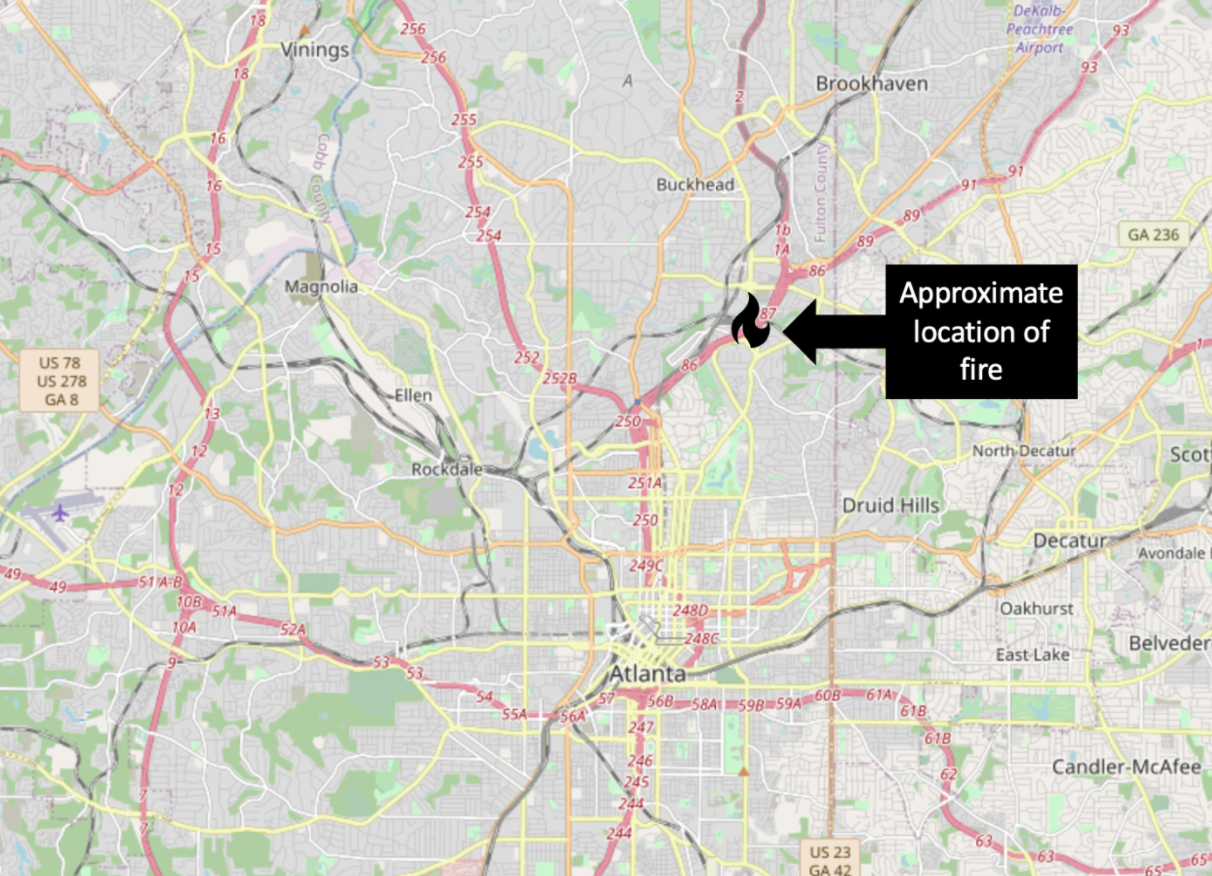
\includegraphics[width=0.75\linewidth]{figures/chapter2/I-85.png}}

\caption{Approximate location of the I-85 / Piedmont Road bridge fire.}\label{fig:i85}

\end{center}
\end{figure}

The section of I-85 that was closed impacted a large, upper income
demographic in the greater
Atlanta area who commuted across the bridge.
As a result, the Georgia Department of Transportation (GDOT) along with
the Governor created a
\$3.1 million incentive program to help motivate project completion ahead
of schedule. The bridge
was originally set to be closed for a period of 10 weeks, however, it re-
opened after just 6
weeks, with construction being completed a month ahead of schedule. The
accelerated finishing
date was estimated to have saved approximately \$27 million in user and
travel time costs
\citep{GDOT2017}. GDOT’s efforts to open the bridge quickly after its
collapse aided in abating negative user costs due to significant travel
time delays that surfaced
due to changes in route choice and assignment.

As a result of the fire, the highway, which had an average daily traffic
count (ADT) of 243,000,
was closed in both directions for a period of about two months. This
closure led to a 30\%
increase in traffic volumes across the entire downtown network, with
increased congestion on side
streets \citep{hamedi2018}. Additionally, the Metropolitan Atlanta Rapid
Transit Authority
(MARTA) experienced a 20\% increase in ridership, likely because many
commuters made mode choice
and route changes. To mitigate this, headways between buses and trains
were decreased to allow
greater passenger volume. MARTA was able to extend service capacity by about 20 percent, adding 142,000 rail miles, 1,100
train hours, 8,202 bus
miles, 512 bus hours, and 2,463 parking spaces in park and ride lots to
help further mitigate the
situation \citep{marta2017, marta2018}. It is likely that MARTA’s efforts
to mitigate the rapid increase in passenger
volumes greatly reduced any negative effects of the bridge
fire on transit services, and helped alleviate other congestion generated by the disaster.

\section{Attempts to Evaluate Systemic Resiliency}

Real world events do occur; however, and it is important for researchers to
base efforts on both theoretical scenarios, and on events that could happen in
the real world. Thus, a number of researchers have conducted studies where real
or fabricated transportation networks are constructed, damaged or degraded, and
then the change to network metrics is evaluated. All of this is done to measure
network performance without
an actual disaster occurring beforehand.
\citet{berdica2002}
attempts
to identify, define and conceptualize vulnerability by envisioning
analyses conducted with
several vulnerability performance measures, including travel time, delay,
congestion,
serviceability and accessibility. Here, Berdica defines accessibility as
the ability for users to
travel between origins and destinations for any number of reasons. She
then uses the performance
measures to define vulnerability as the level of reduced accessibility due
to unfavorable
operating conditions on the network. In particular, Berdica identifies a
need for further
research toward developing a framework capable of investigating
reliability of transportation
networks.

In this section we will examine several attempts by numerous researchers
to do precisely this,
using different measures of network performance. A consolidation of this
discussion is summarized
in Table \ref{tab:authortable}, namely the methods that different researchers have
used in examining network
performance under duress. The measures can be consolidated into three
basic families:

\begin{itemize}
	\item \textbf{Network connectivity}: How does damage to a network
	diminish the connectivity
between network nodes?
	\item \textbf{Travel Time analysis}: How much do shortest path travel
	times between origins
and destinations increase on a damaged network?
	\item \textbf{Accessibility analysis}: How easily can the population
	using the damaged
network complete their daily activities? This in turn can be evaluated in a number of ways as explained by \citet{dong2006}.
\end{itemize}

The following sections discuss relevant studies in each group; Table
\ref{tab:authortable} consolidates these studies by year and labels them
with
an applicable group.

\begin{table}

\caption{\label{tab:authortable}Attempts to Evaluate Systemic Resiliency}
\centering
\begin{tabular}[t]{rll}
\toprule
Year & Author & Performance Metric\\
\midrule
2004 & Geurs and Van Wee & Accessibility (isochrone, gravity, logsum)\\
2006 & Dong et al. & Accessibility\\
2006 & Koppelman \& Bhat & Accessibility (isochrone, gravity, logsum)\\
2007 & Abdel-Rahim et al. & Network Connectivity\\
2007 & Berdica \& Mattson & Network Connectivity\\
\addlinespace
2008 & Taylor, M. & Accessibility (logsum)\\
2010 & Peeta et al. & Travel time and cost\\
2010 & Geurs et al. & Accessibility (logsum)\\
2010 & Jenelius, E. & Network Connectivity\\
2010 & Levinson and Zhu & Travel time and cost\\
\addlinespace
2010 & Zhu et al. & Travel time and cost\\
2011 & Agarwal et al. & Network Connectivity\\
2011 & Ip \& Wang & Network Connectivity\\
2011 & Serulle et al. & Travel time and cost\\
2011 & Ibrahim et al. & Travel time and cost\\
\addlinespace
2011 & Xie and Levinson & Accessibility (isochrone)\\
2012 & He and Liu & Travel time and cost\\
2012 & Masiero \& Maggi & Accessibility \\
2013 & Omer et al. & Travel time and cost\\
2014 & Osei-Asamoah \& Lownes & Network connectivity\\
\addlinespace
2014 & Guze, S. & Network connectivity\\
2015 & Zhang et al. & Network connectivity\\
2015 & Jaller et al. & Travel time and cost\\
2015 & Xu et al. & Network connectivity\\
2016 & Nassir et al. & Accessibility \\
\addlinespace
2016 & Winkler, C. & Accessibility (gravity)\\
2017 & Ganin et al. & Accessibility (gravity)\\
2019 & Vodák et al. & Network connectivity\\
2019 & Hackl and Adey & Network connectivity\\
\bottomrule
\end{tabular}
\end{table}

\subsection{Network Connectivity}

Graph theory is the mathematical study of networks of nodes connected by
edges (links). Within
this discipline are the related concepts of network vulnerability and
connectivity that have been
accessed by researchers. In these studies, researchers tend to define
critical links as those
that connect to many other nodes (directly or indirectly), or as links
whose loss isolates a
number of nodes from the rest of the network.

\citet{abdel2007} developed a multi-layered graph to examine the resiliency
of the traffic
signal control system in Boise, Idaho. The researchers determined which
traffic signals would be isolated by a failure to a particular power
substation,
and consequentially the percent of travel paths that would experience
diminished
levels of service. The research highlights the degree to which interrelated
infrastructure systems --- power, telecommunications, and transportation --
-
depend on each other, though the researchers did not attempt to look at the
connective resiliency of the transportation network directly.

\citet{agarwal2011} present a method to represent a transportation network
as a
hierarchical or cluster graph that can be analyzed more directly for
vulnerabilities. Clusters are formed as groups of links and nodes become
isolated from each other. Clusters of links and nodes are then grouped
together more tightly by including nearby clusters, which creates a
``zoomed out'' model where small clusters begin to act as nodes or links.
In the study, links in the system are damaged, and the resulting
connectedness of the network is evaluated. One scenario of importance
noted by the authors, however, is that a maximal failure consideration where a
node
is entirely isolated from the network is unlikely in a real-world network
with
multiple paths of connectivity. The authors do discuss the importance of
having damaged networks with high levels of functionality. \citet{vodak2019}
on the other hand, develop an approach to identify
critical links in a network by searching for the shortest independent
loops in the network. An independent loop is essentially a way to travel
between an origin and a destination over any number of alternative routes.
The algorithm progressively damages one or more links
between iterations to determine if nodes become isolated, or cut off from
the
network. If a node becomes easily isolated or has a higher likelihood of
becoming isolated, then there is a higher degree of vulnerability present
in the
network. This method can both identify critical links in individual
networks, as
well as provide a means to quantitatively compare networks.

\citet{ip2011} address this shortcoming through the concept of
\textbf{friability}, or
the reduction of capacity caused by removing a link or node, in order to
determine criticality of individual links. The methodology relies on the
ability
to determine the weighted sum of the resilience of all nodes based on the
weighted average of connectedness with other city nodes in the network. The
authors determine that the recovery of transportability between two cities
largely depends on redundant links between nodes. The authors also comment
that
most traffic managers are more concerned with the friability of single
links
rather than the friability of multiple links or an entire system. This suggests
that planners and managers may not be considering the importance of
understanding the impacts of widespread, all-inclusive disaster scenarios.

\citet{guze2014} conducts a review of the known uses of graph theory
(a possible application of resiliency) before
reviewing several
other multi-criteria optimization methods.
Graph theory is the study of pairwise objects, and is
useful for identifying
shortest path, network connectivity, and other methods of network
optimization. Graph theory
supports the idea of resilience through recovery as well as operability through crisis
because of how it
represents networks with links and nodes, and the theory's ability to identify next
shortest paths in the
case of disaster. Guze’s methodology
involves an
analysis of the knapsack problem which is a combinatorial optimization problem.
Specifically, Guze focuses on flow
theory in transportation
systems and identifying a method to find the best graph solution. Guze’s
greatest contribution to transportation research
is a simplified method
for determining shortest path route options on simple networks.

\citet{osei2014} adopt a network analysis methodology that is able to
analyze
resilience of transportation networks. In this
article, the authors evaluate resilience by comparing the biological
network of a common mold
with a rail network. The network for both the mold and the railway are
complexly connected. The giant component is given by:

\begin{equation}
	\Phi = \frac{E'}{ E}
\end{equation}

\noindent where $\Phi$ represents the giant component, $E$ represents the
level of connectivity before the network is damaged, and $E'$ represents the
level of network connectivity after the network is damaged. After the giant component
is found, network efficiency is determined using the
shortest path available. By combining both the ratio of link connections and
network efficiency, the authors are able to draw comparisons between two
complex networks. Ultimately, the authors conclude that a denser, highly
interconnected network will perform better if a link is cut due to a larger giant component value.

\citet{zhang2015} investigates the role of network topology, or the physical
layout of the network in a geographic location.
The authors provide several examples of network topology types including
hub and spoke, grid, and
ring networks. After computing resilience indexes, or general resilience
levels of each type of
network topology, the authors determine that metrics such as throughput,
connectivity and average
reciprocal distance increase with greater lineage, however they decrease as
networks become
more widespread. This is likely because larger networks have fewer, less dense node
connections, and
therefore are less redundant.

Each of the graph theoretical approaches discussed in this section tend to break
down in efficiency or connectivity as networks become larger. Real-world
networks are typically extremely large, with nodes and links numbering in the
hundreds, if not thousands. Thus, the connectivity of a node may be high though
connectivity may not be an accurate representation of a node's importance.

\subsection{Changes in Travel Time}

Highway system network failures --- in most imaginable cases --- degrade
the
shortest or least cost path, but typically do not eliminate all paths.
The degree
to which travel time increases when a particular link is damaged, or a node
becomes isolated, could
provide an estimate of the criticality of that link or node. If a link or node
becomes completely isolated, the travel time to that node or link would
increase indefinitely. Thus, ensuring total isolation of a node or link does
not occur becomes highly important to network resiliency in terms of graph theory.

\citet{Berdica2007} attempt to examine what the effects of road
degradation on Stockholm's transportation network would be if one or more
chokepoints were to become damaged or all-together inundated. The authors
sought to determine how interruptions affect the system, and how overall
system performance was affected. Users in this method were only given the
choice of an alternate route, and the authors acknowledge that this is not
entirely reasonable in a real world situation. This method purely attempts
to quantify delay experienced by users compared to the original
equilibrium state, but does make an attempt to determine a monetary value
associated with closure or degradation.

\citet{Jenelius2010} attempts to examine the importance of the link that
becomes critical only after partial network degradation, or redundancy
importance. This measure is primarily flow-based. In the presented context,
flow-based measures aim to analyze and evaluate changes in the number of
vehicles using a route given adverse circumstances on the network.


\citet{peeta2010} construct a model to efficiently allocate
highway maintenance and emergency response resources at locations throughout a
network. Each link in the sample network was
assigned a specific failure probability based on resource allocation;
the model evaluated the increase in travel time resulting from a broken
link. The authors applied a Monte Carlo simulation  of multiple scenarios,
which revealed resource allocation plans with the least network degradation,
and thus which links were most critical to the network's operations.

\citet{serulle2011} clarify variables related to resiliency
of transportation networks including average delay and transport cost,
adjusting interactions,
and increasing metric transparency. The authors employ a methodology
capable of quantifying
resiliency using a fuzzy interference approach – an approach meant to use
imprecise or vague data
– that relates physical and performance characteristics. The used approach
is able to determine a
resiliency index that supports comparative and sensitivity analyses.
Accessibility data, including
available road capacity, road density, alternate route proximity, average
delay, transport cost,
and average speed reduction, are analyzed for importance to the integrity
of the network.

\citet{ibrahim2011} provide an approach for determining
vulnerability of infrastructure by estimating the cost of single link
failure based on the increase in shortest path travel time due to
increased congestion
levels. The authors propose a hybrid heuristic approach that calculates the
traditional user-equilibrium assignment for finding the first set of
costs, and
then fixes those costs for all following iterations to determine the
effects of
failure on overall travel time of the system.

\citet{omer2013} proposes a methodology for assessing the resiliency of
physical infrastructure
during disruptions. To do this, the authors use a network model to build
an origin-destination
matrix that allows initial network loading and analysis. Omer’s model uses
several metrics, but
the main metric used to determine resiliency is the difference in travel
time between a disturbed
and undisturbed network. Omer’s framework is applied to an actual network
between New York City
and Boston for analysis. Changes in demand, travel time, mode choice and
route choice are tracked
for analysis. Omer’s framework supports operability of transportation
networks due to the way it
analyzes networks experiencing suboptimal circumstances. The author's work
identifies key
parameters that should be measured to assess resiliency during disruptive
events.

\citet{jaller2015} seeks to identify critical infrastructure based on
increased travel time or
reduced capacity due to disaster. The proposed methodology utilizes user-
equilibrium to determine
proper initial network loading. Then the shortest path between one origin
and one destination
can be identified. To implement damage to the network, a link is cut, and
then the next shortest
path is found. This process is followed for all links in the system in
order to determine a sense
of the criticality of each link to network resiliency. The analysis is
carried out for each O-D
pair, and the nodes with greatest change in travel time are determined to
be the most critical.
Jaller’s methodology allows traffic managers to identify critical paths
for mitigation purposes
before the occurrence of disaster through careful analysis.

A primary limitation with increased travel time methodologies is that they
ignore the other possible ways a population might adapt its travel to a
damaged
network. Some people may choose other modes or destinations, and it is
possible
that some previously occurring trips might be canceled entirely. It may also be
prudent to consider how access changes, and evaluate changes in user choice
based purely upon accessibility.

\subsection{Changes in Accessibility}
\label{sec:cacc}
In a travel modeling context, \textbf{accessibility} refers to the ease
with which
individuals can reach the destinations that matter to them; this is an
abstract
idea but one that has been quantified in numerous ways. \citet{dong2006}
provide a
helpful framework for understanding various quantitative definitions of
accessibility that we will simplify here. The most elementary definition of
accessibility is whether a destination is within an \textbf{isochrone}, or
certain
distance. This measure is often represented as a count, e.g., the number
of jobs
reachable from a particular location within thirty minutes travel time by a
particular mode. Mathematically,

\begin{equation}
A_i = \sum_{j} X_j I_{ij}; I_{ij} = \begin{cases}  1 \text{ if } d_{ij}
\leq D\\
0 \text{ if } d_{ij} > D \end{cases}
	\label{eqn:isochrone}
\end{equation}

\noindent where the accessibility \(A\) at point \(i\) is the sum of the all the
destinations \(X\) at other points \(j\). \(I_{ij}\) is an indicator
function equal to
zero if the distance between the points $d_{ij}$ is less than some asserted
threshold (e.g., thirty minutes of travel time). By relaxing the
assumption of a
binary isochrone and instead using the distance directly, we can derive the
so-called gravity model,

\begin{equation}
A_i = \sum_{j} X_j f(d_{ij})
  \label{eqn::gravity}
\end{equation}

\noindent where the function $f(d_{ij})$ is often a negative exponential with a
calibrated
impedance coefficient. An extension of the gravity model is to use the
logsum
term of a multinomial logit destination choice model,

\begin{equation}
A_i = ln\sum_{j} \beta_d(d_{ij}) + X_j\beta
  \label{eqn:logsum1}
\end{equation}

\noindent where the parameters $\beta$ are estimated from choice surveys or
calibrated to
observed data. The logsum term has numerous benefits outlined by
\citet{handy1997}
and \citet{geurs2004}; namely, the measure is based in actual choice
theory, and
can include multiple destination types and travel times by multiple
different modes.

\citet{geurs2004} provide a review of accessibility measures such as those
above, up to
2004 in a literature review done at the time. Of the papers they reviewed,
Vickerman (1974), Ben-Akiva and Lerman
(1979), and Geurs and
Ritsema van Eck (2001), used isochrone type methods. Stewart (1947),
Hansen (1959), Ingram (1971), Vickerman (1971), and Anas (1983) used gravity
style models, and
Neuburger (1971), Leonardi (1987),
Williams and Senior (1978), Koenig (1980), Anas (1983), Ben-Akiva and Lerman
(1985), Sweet
(1997), Niemier (1997), Handy and Niemier (1997), Levine (1998), and Miller
(1999) used or
suggested logsums. They highlight the importance of using person-based
measures such as these in
evaluating network vulnerability and resiliency.

\citet{taylor2008} applied logsum-derived accessibility analysis to
evaluate the consequences of a tunnel failure in Adelaide, Australia. An
accessibility framework capable of evaluating the change in accessibility
for a multimodal urban network was designed. The designed framework is
capable of determining the ability of an individual to access an activity.
Taylor's framework captures five types of choice: activity, time period,
trip-base, location, and mode choice, with key features being activity
choice and trip-base (the origin point of a trip). Each of these choice
models use typical multinomial logit models (MNL), with the exception of
the mode choice model, which uses a nested MNL model. The main choice
considered in the framework is activity choice followed by trip choice.
Taylor's proposed framework has been applied to an existing activity based
choice model for the Adelaide region, however, the framework operates
independently from the parent model.

Using the developed framework, Taylor calculates an ``inclusive value'' (IV)
and ``consumer surplus'' (CS) values.. Both the IV and CS values are vital to
determining the benefit or dis-benefit
associated with the change experienced by users in the individual model
scenarios considered.

Taylor's accessibility framework, applied as a separate or connected module to
the Adelaide model, estimates the IV and CS values using a logsum.
These values allow Taylor to show that more disruption occurs near the
failed link than occurs farther away. Additionally, Taylor is able to show
that a greater cost (nearly 40 times greater) is experienced by those who
live in a TAZ near the link than by those who live in a TAZ located
farther away from the failed link. Taylor's framework primarily
investigates accessibility on a network for a large city,
but could easily be applied on a larger scale.

In the Adelaide model, Taylor breaks one link and
then calculates the difference in IV and CS values using:

	\begin{equation}
		E(CS) = \frac{1}{\alpha} \log (\sum_{j = 1}^{J} \exp (I_j)) + \beta
			\label{eqn:taylor}
	\end{equation}

\noindent where the \(\alpha\) represents the negative of the coefficient of time or cost from the utility function,
and \(\beta\) is an unknown constant that represents the difference between the actual value of CS and the estimated value.
The \(I_j\) term represents the observable attributes of the possible utility. 

Taylor's research highlights the possibility for a comprehensive model capable
of succinctly measuring the dis-benefit caused by a degraded network.
Taylor continues by stating that traffic network simulation models
could be considered for future research. Some of the key needs for
future research specifically highlighted at the conclusion of Taylor's article include:

	\begin{itemize}
		\item efficient algorithm development
		\item improved vulnerability metrics
		\item use of network vulnerability indicators in studies of critical
		infrastructure and the implications of network degradation
		\item improved techniques for identifying network weaknesses
	\end{itemize}

\noindent Several authors employ various types logit models in their research,
or attempt to develop a methodology specifically for use analyzing disrupted networks.

\citet{Masiero2012} use logit-based calculations to determine the Value of
Time (VOT) associated with the closure of a road in terms of cost, time,
and punctuality for freight transport. In order to properly determine the
VOT of route closure, the authors also use a method provided in
\citet{koppelman2006} which uses model derived coefficients and values to
determine the cost of an alternative. The authors implemented their
model on a network consisting of a single travel corridor that has
experienced long (1 week to 2 months or more) closures in the past.

\citet{Nassir2016} applies a nested logit model to examine a transit
network in Australia. The main contribution in \citet{Nassir2016} is an
improved methodology for calculating accessibility measures related to
transit, accomplished by developing a method to account for diversity
information. The authors do note, however, that this measure is best applied
to models with complex transit systems that serve large portions of the
community. One important observation, however, is that users do not always
choose the fastest route, nor do they always choose the route with the
highest utility. \citet{He2012} take another look at the after effects of
the I-35W bridge collapse previously discussed. A key contribution of
\citet{He2012} is that people often initially base route choice on what they
assume will be best based on past experience. So, over time, users
adjust their route choice to an altered network. The true implication here
is that users do not automatically choose the best new route given an
altered network, it takes users time to learn how the new network
functions.

\citet{winkler2016} proposes a travel demand model that is valid for all
networks,
especially those with more than one constraint.
Winkler’s methodology
utilizes a
model that uses production, distribution, and mode choice as inputs. The
methodology shows that models can be used to help determine outputs for
multi-constraint Multinomial Logit Models (MNL). Logsums like Winkler’s
also allow for consumer surplus calculations,
or utility, to be estimated across the transportation network
being modeled.

\citet{ganin2017} attempt to investigate resiliency through a disruption
of 5\% of the roadways
in 40 urban networks within the United States. The employed methodology
determines that Salt Lake
City has the most resilient transportation network while Washington D.C.
has the least resilient.
This determination is based on a comparison of simple gravity models of the identified networks after links are
damaged versus before.
The authors work three factors into each model, which account for
differences in car-
truck ratios, average speed, and average vehicle length. Using a gravity
model to determine commuting patterns, the authors were
able to estimate the average
annual delay per commuter. They used this to determine network efficiency.
\citet{ganin2017} noted that
traffic delay times (or the travel time caused by a closure) increase
significantly as road segments are broken.

\section{Summary}

The lessons learned from the events in Minneapolis and Atlanta demonstrate
that when
transportation networks are damaged or degraded by link failure, multiple
changes result. Traffic
diverts to other facilities and other modes, and some people make
fundamental changes to their
daily activity patterns, choosing new destinations or eliminating trips
entirely. Numerous other
researchers have identified methodologies to capture the effects, or at
least have made quality attempts to capture the costs of these
potential changes to accessibility in modeled crisis events. Some researchers
have even applied logit-based models to small scale activity based models.
From this extensive review of existing literature, we are able to see that no
one has attempted to apply a logit-based choice model on a statewide level.
